\documentclass[a4paper,10pt]{article}

\usepackage[bottom=0.5cm]{geometry}

%A Few Useful Packages
\usepackage{marvosym}
\usepackage{fontspec} 					%for loading fonts
\usepackage{xunicode,xltxtra,url,parskip} 	%other packages for formatting
\RequirePackage{color,graphicx}
\usepackage[usenames,dvipsnames]{xcolor}
\usepackage[big]{layaureo} 				%better formatting of the A4 page
% an alternative to Layaureo can be ** \usepackage{fullpage} **
\usepackage{supertabular} 				%for Grades
\usepackage{titlesec}					%custom \section

%Setup hyperref package, and colours for links
\usepackage{hyperref}
\definecolor{linkcolour}{rgb}{0,0.2,0.6}
\hypersetup{colorlinks,breaklinks,urlcolor=linkcolour, linkcolor=linkcolour}
\urlstyle{same}

%Defined width table colums that work like l, c and r.
\usepackage{array}
\newcolumntype{L}[1]{>{\raggedright\let\newline\\\arraybackslash\hspace{0pt}}m{#1}}
\newcolumntype{C}[1]{>{\centering\let\newline\\\arraybackslash\hspace{0pt}}m{#1}}
\newcolumntype{R}[1]{>{\raggedleft\let\newline\\\arraybackslash\hspace{0pt}}m{#1}}
\newcolumntype{D}{>{\raggedleft\let\newline\\\arraybackslash\hspace{0pt}}m{1.51cm}}

\usepackage{tabu}	%For distributing remaining tab space evenly

%FONTS
\defaultfontfeatures{Mapping=tex-text}
%\setmainfont[SmallCapsFont = Fontin SmallCaps]{Fontin}
% modified for Karol Kozioł for ShareLaTeX use
\setmainfont[
SmallCapsFont = Fontin-SmallCaps.otf,
BoldFont = Fontin-Bold.otf,
ItalicFont = Fontin-Italic.otf
]
{Fontin.otf}

\newfontfamily\namefont{Times New Roman}%Quattrocento-Regular.ttf}

\usepackage{anyfontsize}	%set any font size (duh)

%%%

%CV Sections inspired by: 
%http://stefano.italians.nl/archives/26
\titleformat{\section}{\Large\scshape\raggedright}{}{0em}{}[\titlerule]
\titlespacing{\section}{0pt}{3pt}{3pt}

%Tweak a bit the top margin
\addtolength{\voffset}{-0.4cm}


%--------------------BEGIN DOCUMENT----------------------
\begin{document}

\pagestyle{empty} % non-numbered pages

%--------------------TITLE-------------
{  \Huge \namefont {\fontsize{35}{0}\namefont C}LAES {\fontsize{35}{0}\namefont A}NDERSSON} \bigskip\par

%--------------------SECTIONS-----------------------------------
%Section: Personal Data
\section{Personlig Data}

\begin{picture}(0,0) 
\put(272,-96){\hbox{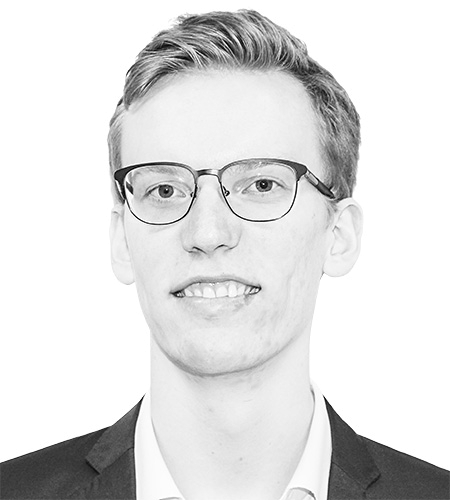
\includegraphics[scale=0.4]{profile}}}
\end{picture}

\begin{tabular}{Dl}
    \textsc{Adress:}	&	 Vänortsvägen 5, Luleå, Sverige \\
    \textsc{Telefon:}		&	 +46 73 763 87 77\\
    \textsc{Email:}		&	 \href{mailto:Claes.Gustaf.Andersson@gmail.com}{Claes.Gustaf.Andersson@gmail.com}\\
    \textsc{Linkedin:}	&	 \href{https://linkedin.com/in/ClaesGustaf}{linkedin.com/in/ClaesGustaf} \\
    \textsc{GitHub:}		&	 \href{https://github.com/Fizzr}{GitHub.com/Fizzr}
\end{tabular}

%\section{Mål}
%{\small Mitt huvudsakliga mål i karriären är att lära mig. Jag vill bli utmanad på ett sätt som tvingar mig att lära mig nya saker och tänka i nya banor. Jag vill bli den bästa i mitt område och vara med att skapa felfria och perfekta lösningar!}

%Section: Education
\section{Utbildning}
\begin{tabular}{D L {\textwidth - 2.7cm}}
\textsc{Jun 2018}	&	\textbf{Datateknik Civilingenjör}\\
\textsc{Aug 2012}	&	 \emph{Informations- and Kommunikationsteknik}. Luleå Tekniska Universitet.\\
			&	{\small Fokus på algoritmer, Design paradigmer, hög nivå av abstraktion, nätverk, och internettjänster och utveckling.}
\end{tabular}


%Section: Work Experience
\section{Arbetserfarenhet}
\begin{tabular}{D L {\textwidth - 2.7cm}}
 \emph{Nu} 	& 	\textbf{Brand Ambassador}	\\
 \textsc{Mar 2015}	&	Academic Work			\\
 			&	{\small Som Brand Ambassador deltar jag på olika typer av event och arbetsmarknadsdagar för att värva kandidater samt stärka Academic Works varumärke. Yrket kräver god förmåga att kommunicera. Arbetsuppgifter innefattar
\begin{itemize}
\setlength{\itemsep}{0pt}
\setlength{\parskip}{0pt}
\setlength{\parsep}{0pt}
	\item Nätverkande
	\item Sälj
	\item Medlemsvärvning
\end{itemize}
} 	\\		

\emph{Nu}	&	\textbf{Bolagsman, Delägare}		\\
\textsc{Sep 2013}	&	DC Technological Innovations HB	\\
 			&	{\small Ett företag bildat i försök att bringa crypto-valutan Bitcoin till universitetet och göra den till den dominerande betalningsmedlet på campus. Numer vilande.}					\\
 			&						\\
\textsc{Aug 2016}	&	\textbf{Junior Utvecklare}		\\
\textsc{Jun 2016}	&	isMobile				\\
			&	{\small Konsultarbete genom Academic Work. Arbetade med att utveckla en demo suite för deras Android Applikations modul. Skrev mestadels i XSLT, HTML, JavaScript, Java samt LaTeX.}	\\
			

\end{tabular}


%Section: Languages
\section{Språk}
\begin{tabular}{Dl}
\textsc{Svenska}		&	Modersmål\\
\textsc{Engelska}		&	Flytande\\
\end{tabular}

\section{Datorkunskap}
\def\arraystretch{1.2}%  1 is the default, change whatever you need
\begin{tabu}to \textwidth{r X[c] X[c] X[c] X[c] X[c]}
\textsc{Traditionella Språk:}	&	C/++/\#	&	 Java		&	Python	&			&		\\
\textsc{Webbutveckling:}		&	 HTML		& 	JavaScript	&	PHP		&	MySQL	& 	CSS	\\
\textsc{Övrigt:}			& 	LaTeX		&	XML		&	XSLT		&	JSON		&	 Git	\\
\textsc{Miljöer:}			&	Android	& 	Unity		&	3ds Max	&	Office		&		\\
\textsc{Rört vid: }			&	Go!		&	 Prolog	&	Haskell	&	Assembly	&	 VHDL
\end{tabu}
\\[0.3cm]

\centering\textsc{ Referenser lämnas på begäran}

\end{document}
